
Randomness can be referred to as the property that a set of information \textbf{cannot be certainly predicted}, where there is no defined and deterministic pattern in how they were sorted or generated. According to Kendall and Babington Smith \cite{489b709a-b56c-3c3f-bfcb-5d1507b7d20e}, it refers, in casual terms, to a method of choice that \textbf{lacks aim or purpose}. In terms of statistics, it takes on more specific definitions closely related to \textbf{probability}, focusing on the aspect of \textbf{statistical frequencies} within the random information and studying their \textbf{degree of uncertainty}, as well as \textbf{judging} whether any given data or sampling method is random or not.

This concept of randomness is the core of many fields, some of which reach a serious and sensitive level. While randomly generated numbers are used in game development and the lottery industry \cite{10.1007/978-981-15-4474-3_4}, there are some crucial uses of it, mainly in the security of information systems \cite{Shanon} and cryptography \cite{Crypto}, where it plays a pivotal role in generating and producing keys and digital signatures for communication protocols used in IoT (Internet of Things) devices to transfer personal and highly confidential materials.

These crucial and highly demanded usages require the random numbers to adhere to a high rate of randomness by assuring some of the main characteristics: \textbf{unpredictability, unreproducibility, and a uniform and equally probable distribution}. In order to achieve that, several schemes have been proposed, designing the structures of \textbf{Random Number Generators (RNGs)}.



\section{Random Number Generators (RNGs) \& True Random Number Generators (TRNGs)}
An \textbf{RNG} is a system that generates numbers with the essential property of unpredictability, using various techniques and algorithms. As a general concept, an RNG can take many forms, such as physical ones like a \textbf{dice}, a \textbf{game wheel}, a \textbf{Galton Board}, or integrated algorithms in a \textbf{classical computer}, or even a \textbf{quantum computer}.

In the previous section, we mentioned the three main features that help judge the randomness of a generated number. By ensuring all these properties in a generation system (automatically applicable to the sampled data), a random number can be referred to as a \textbf{True Random Number}, and its generator as a \textbf{True Random Number Generator (TRNG)}. These features are:

\begin{itemize}
    \item \textbf{Unpredictability}: In a sequence of truly generated random numbers, the next generated value cannot be guessed, and each generation is independent of the previous values. This means that the next value cannot be determined based on the previously generated values. \textbf{Note}: The absence of this feature collapses the randomness of the generator (the generator is not random).
    
    \item \textbf{Unreproducibility}: For large number sequences, true random number generation cannot be reproduced. As the length of the sequence increases, the likelihood of generating two identical sequences decreases and converges to zero.
    
    \item \textbf{Uniform Distribution}: After a long series of true random generations, all possible basic values that the generator could produce should appear with equal likelihood, with no bias toward any specific value. This also applies to their possible combinations, which should appear equiprobably. \\
    \textit{E.g.}: In a generated bitstream, the probability of bits being 0 and the probability of bits being 1 should be equal but also, the probability of the two-bit words (\textbf{00}, \textbf{01}, \textbf{10}, \textbf{11}) should also be equal and so on for all possible combinations.
\end{itemize}



\section{Pseudorandom Number Generators PRNGs}
Nowadays, most of the random numbers used in cryptographic algorithms to encode our sensitive online materials (bank accounts, passwords, data sharing, and network tokens) are generated using classical computers and complicated algorithms. It may sound strange, but for a classical computer, no matter how advanced it is, it is difficult to get a computer to do something by chance. A computer running a program follows its instructions blindly and is therefore completely predictable \cite{haahr1999random}.

These kinds of generators are called \textbf{Pseudo-Random Number Generators} (PRNGs). They use discrete algorithms and calculations starting from an initial number called the \textbf{Seed}, such as the \textbf{Linear Congruential Generator (LCG)} described in \cite{LCG}. This method uses the following formula:
\begin{equation}
X_{i+1} = (aX_i + c) \mod M
\end{equation}
where \( a \) is a multiplier relatively prime to \( M \), and \( c \) is an increment, both chosen \textbf{appropriately}. Then, starting at a random seed \( X_0 \), the sequence \( \{X_i\} \) is generated.

The method successfully passes several randomness tests, but it breaks through the principle of \textbf{Unreproducibility}. Knowing the value of the seed (if it is leaked or somehow stolen) will allow one to reproduce the exact same random numbers and predict the next ones. We show in Appendix One how the same seed would reproduce the exact same sequence, and how this could break the encryption methods. Thus, the generated numbers appear to be random, but they are not.

Several other advanced algorithms have been proposed in order to reduce these risks, like the \textbf{Mersenne Twister based on linear shift feedback registers} \cite{matsumoto_1998_mersenne}, and \textbf{One-Time Pad (OTP) encryption} \cite{OTP}. These achieve good likelihood of randomness, but the fact that they are reproducible reduces the scope of their use.


\section{Quantum Random Number Generators (QRNGs)}
 A lot of schemes have been presented to create a True Random Number Generator that outputs true random numbers within the three aforementioned characteristics. Since \textbf{deterministic calculations could never generate a true random number}, some of the proposed schemes exploit and utilize \textbf{the randomness in physical noise} by sampling and processing a \textbf{hardware source of entropy} outside the computer. This can vary from using simple sources, like little variations in somebody’s mouse movements \cite{mouse}, to more advanced physical entropy sources, such as radiation \cite{radiation}, stable random telegraph noise \cite{RTN}, and different schemes that use \textbf{the basic randomness property features of various quantum systems} like Boson Sampling-based generators \cite{shi_Twa3na}, photon counting generators \cite{photonic}, generators based on quantum vacuum fluctuations \cite{Vaccum}, and others introduced and explained in \cite{OtherQrngs}.

These proposed schemes use \textbf{the physical uncertainty} of the systems as \textbf{entropy sources}. The raw extracted data from these methods often \textbf{exhibit statistical defects}, yet it \textbf{remains random} and in order to correct these defects, \textbf{deterministic algorithms} are applied to the generated data from the physical entropy source. 

The use of these deterministic concepts \textbf{does not affect the true randomness} of the generator, since the randomness source itself is \textbf{unreproducible}, and the post-processor is simply a method of \textbf{correction and extraction of maximum possible true randomness}.


Quantum Random Number Generators uses the same scheme of Entropy source-Post processor as you can see in Fig. \ref{fig:quanta}. 

\begin{figure}
\centering
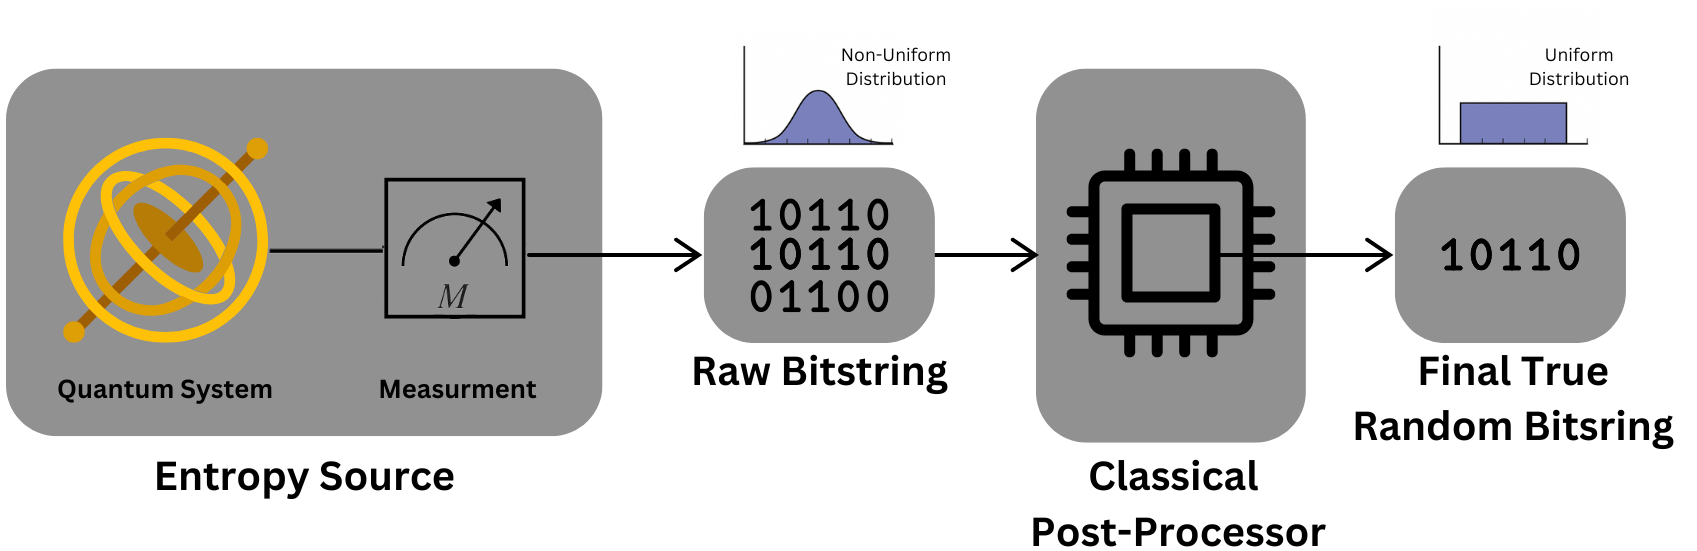
\includegraphics[width=16.5cm]{figures/Quantum System.png}\vspace{-0.2cm}
\caption{Quantum Random Number Generator (QRNG) Process}
\label{fig:quanta}
\end{figure}

\section{Post Processors (PP)}
\noindent
\begin{tcolorbox}[colframe=blue!20!white, colback=yellow!10!white, coltitle=black, title=Note]
     In this work, we will consider that Random Number Generators (RNGs) produce bitstrings, often referred to as \textit{bitstreams}, of length \(N\), where each atomic value can either be \(0\) or \(1\) \& We will model the systems and approaches based on this structure.
\end{tcolorbox}

In our context, \textbf{Post Processors (PP)} are \textbf{deterministic classical methods} applied to the \textbf{raw output} of an entropy source that generates random but \textbf{imperfect data}. These methods aim to \textbf{correct statistical defects} in the raw data to ensure that the final output meets true randomness standards. Several approaches have been proposed to address different types of defects observed in bitstreams. Below, we outline two main defects that post-processors aim to address: \textbf{Bias} and \textbf{Autocorrelation}.

\subsection{Bias}  
When examining the raw output of the entropy source, we can notice that the generated bitstream exhibits bias toward one of the atomic possible outcomes at various stages:  
- \textbf{1-bit bias:} The probability that a single bit is 0 (or 1) is higher than the probability that it is 1 (or 0, respectively).  
- \textbf{2-bit bias:} At the 2-bit stage, the probability that all the possible 2-bit patterns (00, 01, 10, 11) aren't equal.  
- \textbf{n-bit bias:} The probability that all the possible n-bit patterns aren't equal, which introduces bias at this level.

To quantify this property, we will use a mathematical measure of randomness: the Shannon Entropy.

\textbf{Shannon Entropy:}  
In our study, we will use a normalized version of the Shannon Entropy function to simplify the interpretation of the results:

\begin{equation}
H(A) = - \frac{1}{n} \sum_{i \in A_n} p_i \log_2 (p_i)
\end{equation}

Where:
\begin{itemize}
    \item \( A_n \) is the set of possible outcomes of \( n \) bits.
    \item \( p_i \) is the probability of the \( i \)-th outcome in \( A \).
    \item \( n \in \mathbb{N}, n \geq 1 \) is the number of bits or bit patterns we are analyzing; \( n \) can be greater than 2.  
    For example, if \( n=1 \), then \( A = \{ 0, 1 \} \); if \( n=2 \), then \( A = \{ 00, 01, 10, 11 \} \); and so on.
\end{itemize}

The value of \( H(A) \) ranges between 0 and 1. 
A value \textbf{close to 1} indicates \textbf{high randomness} (maximum entropy), meaning the bitstream is \textbf{unbiased} and \textbf{random}. Conversely, a value \textbf{close to 0} indicates \textbf{low randomness} (minimum entropy), meaning the bitstream is not random and biased.


\subsection{Autocorrelation (AC)}  
In a bitstream, AutoCorrelation (AC for short) measures the degree of \textbf{correlation} and \textbf{dependency} between the bits of \textbf{the same bitstream} at a \textbf{delay} (or \textbf{lag}) of \( k \).  
It indicates how likely it is that a bit at position \( i \) \textbf{will influence the nature of another bit} at position \( i+k \).

In our study, we are going to quantify the autocorrelation using the autocorrelation coefficients \( \phi_k \).

\textbf{Autocorrelation Coefficient Formula:}  
The autocorrelation coefficient at lag \( k \), denoted as \( \phi_k \), is calculated using the following formula:


\begin{equation}
\phi_k = \frac{\text{Cov}(X_i, X_{i+k})}{\sigma_X^2} = \frac{\sum_{i=1}^{i = n - k}[(X_i - \mu)(X_{i+k} - \mu)]}{\sum (X_i - \mu)^2}
\end{equation}

Where:
\begin{itemize}
    \item \( X_i \) represents the value of the bitstream at position \( i \), and \( X_{i+1} \) represents the value of the bitstream at position \( i+1 \)
    \item \( \text{Cov}(X_t, X_{t+k}) \) is the covariance between the bits at positions \( t \) and \( t+k \).
    \item \( \mu \) is the mean of the bitstream.
    \item \( \sigma_X^2 \) is the variance of the bitstream.
\end{itemize}

For \( k=1 \), the autocorrelation coefficient can also be calculated using \textbf{Pearson’s formula}:

\begin{equation}
\phi_1 = \frac{p_{11} p_{00} - p_{10} p_{01}}{p_1 p_0}
\end{equation}

Where:
\begin{itemize}
    \item \( p_{11}, p_{00}, p_{10}, p_{01} \) denote the probabilities (or frequencies) of each 2-bit pattern occurring in the bitstream.
    \item \( p_1 \) and \( p_0 \) are the probabilities of individual bits being 1 or 0, respectively.
\end{itemize}

The autocorrelation coefficient \( \phi_k \) takes values between -1 and 1 for any lag \( k \):
\begin{itemize}
    \item \( \phi_0 = 1 \): The autocorrelation at lag 0 is always 1 because a bit is always identical to itself.
    \item \textbf{Positive Autocorrelation} (\( \phi_k > 0 \)): The bits at positions \( i \) and \( i+k \) tend to be similar. For example, if the \( i \)-th bit is 0, the \( (i+k) \)-th bit is more likely to be 0 as well.
    \item \textbf{Negative Autocorrelation} (\( \phi_k < 0 \)): The bits at positions \( i \) and \( i+k \) tend to alternate. For example, if the \( i \)-th bit is 0, the \( (i+k) \)-th bit is more likely to be 1, and vice versa.
    \item \( \phi_k \) approaching 0 indicates that the bitstream becomes decorrelated for that lag, reflecting higher randomness and independence.
\end{itemize}

\textit{\textbf{Note: Implementation of the quantifying functions (Entropy and Autocorrelation) using Python is included in the Appendices.} }

 
In order to overcome the above shortcomings, several post-processing approaches were proposed. Alongside the aforementioned metrics, we also introduce the \textbf{Extraction Efficiency} Metric (ExE for short), which evaluates the \textbf{output bitstream length} of the Post Processor over the \textbf{input bitstream length} (the raw one we obtained from the \textbf{entropy source}). Its formula can be written as:

\begin{equation}
    \text{ExE} = \frac{\text{len}(Output)}{\text{len}(Input)}
\end{equation}

Based on this, and as mentioned in the work of Zhang et al. in \cite{dede}, we can distinguish 3 types of postprocessors:

\begin{itemize}
    \item \( \text{ExE} < 1 \) => (Output size \textbf{is less} than the input size), such as the simplest XOR function and the most common method: the Von Neumann method, introduced by John von Neumann in 1951 in \cite{von_1951_various}.
    \item \( \text{ExE} = 1 \) => (Output size \textbf{is the same} as the input size), such as Linear Feedback Shift Registers (LFSR) \cite{LSFR} and Markov Chains \cite{markov}.
    \item \( \text{ExE} > 1 \) => (Output size \textbf{is greater} than input size), such as the middle square method \cite{MSMeth}
\end{itemize}

Each of the above-mentioned methods can achieve different results in terms of bias and autocorrelation.

\textbf{\textit{Note: The implementation of the ExE function in python is included in the Appendecies}}

\noindent Let us examine the ones we will need later in this study:

\subsection{The Von Neuman PP}

The Von Neumann post-processing method \cite{von_1951_various} relies on \textbf{discarding some information} from the bitstring generated by the entropy source to construct a \textbf{new unbiased one}.

The method relies simply on devising the given bitstrings into pairs of \textbf{2 bits} and than apply the following mapping:

\begin{equation}
    \quad 00 \rightarrow \Lambda , \quad 01 \rightarrow 0 , \quad 10 \rightarrow 1 , \quad 11 \rightarrow \Lambda
\end{equation}

where \( \Lambda \) represents no output digit, so by discarding the pairs that contains similar bits which produces the biasdness in the results we can achieve better results.

The highest output rate that can be achieved using the Von Neumann Post Processor (PP) is limited to 25\% of the input rate (ExE = 0.25), and it decreases with the input bias \cite{zonga}.

Several \textbf{variations} with improvements to the original method's throughput have been introduced, such as the N-bits Von Neumann procedure proposed by Peter Elias \cite{peter}. While using \textbf{4 bits}, it achieved an output rate of 40.6\%, and with \textbf{8 bits and a waiting strategy}, it reached a 62.5\% output rate \cite{zonga}. Another variation is the Iterating Von Neumann method proposed by Yuval Peres \cite{yuval}. Each of these methods aims to increase the rate of the Von Neumann post-processor while preserving the unbiasedness of the output.

The Von Neumann Post Processing technique is well known for its ability to achieve zero bias with a minimum entropy guarantee, but at the cost of throughput. Additionally, the input must be independent and uniformly biased (the bias is fixed), and this method, along with its variants, cannot solve or reduce the autocorrelation in the input. \cite{dede}.

\textbf{\textit{Note: The implementation of the Classical Von Neumann function in python is included in the Appendecies}}

\subsection{The Markov Chain PP}  
Discrete-Time Markov chains help determine \textbf{the next state} of a system based on the knowledge of \textbf{the previous one}. This Markov model can be constructed by having \textbf{a finite space} of states (in our case, the number of states is the number of possible combinations according to \( M \), the size (length) of a single state that a Markov chain can work through, which is \( 2^M \)), a \textbf{transition probability matrix} that indicates the probabilities of moving from one state to another, and \textbf{an initial state} from which we can sample the next ones.  

Following this model, we can \textbf{generate an autocorrelated bitstring} with a defined autocorrelation coefficient.  

As an example, consider a Markov chain for \( M=1 \), where the possible states are 0 and 1. We denote the transition probabilities by \( T_{ij} \), where \( i \) represents the previous state and \( j \) the next state. For instance, \( T_{01} \) denotes the probability that the next bit is 1 if the previous one is 0, and so on.  

We can gather the transition probabilities into a transition matrix:  
\begin{equation}
TransitionMatrix = 
\left[\begin{array}{cc}
T_{00} & T_{01} \\
T_{10} & T_{11} 
\end{array}\right]
\end{equation}

\noindentThese transition probabilities follow the constraints: \( T_{00} + T_{01} = 1 \) and \( T_{10} + T_{11} = 1 \).  

\noindent The described scheme is illustrated in Fig. \ref{fig:MKV1}. 

\newline


Probabilities of each bit in a generated bitstring that follows the proposed model will be:

\begin{equation}
[P_0, P_1] = \left[ \frac{T_{01}}{1 + T_{01} - T_{11}}, 1 - \frac{T_{01}}{1 + T_{01} - T_{11}} \right]
\end{equation}

So:

\begin{equation}
P_1 = \frac{T_{01}}{1 + T_{01} - T_{11}}, \quad P_0 = 1 - P_1
\end{equation}

And:

\begin{equation}
\phi_1 = T_{11} - T_{01}, \quad \phi_k = (T_{11} - T_{01})^k = \phi_1^k
\end{equation}

with \( k \) being the lag of the autocorrelation function.

For more proof and explanation, check \cite{dede}.

\begin{figure}[h]
    \centering
    \begin{minipage}{0.45\textwidth}
        \centering
        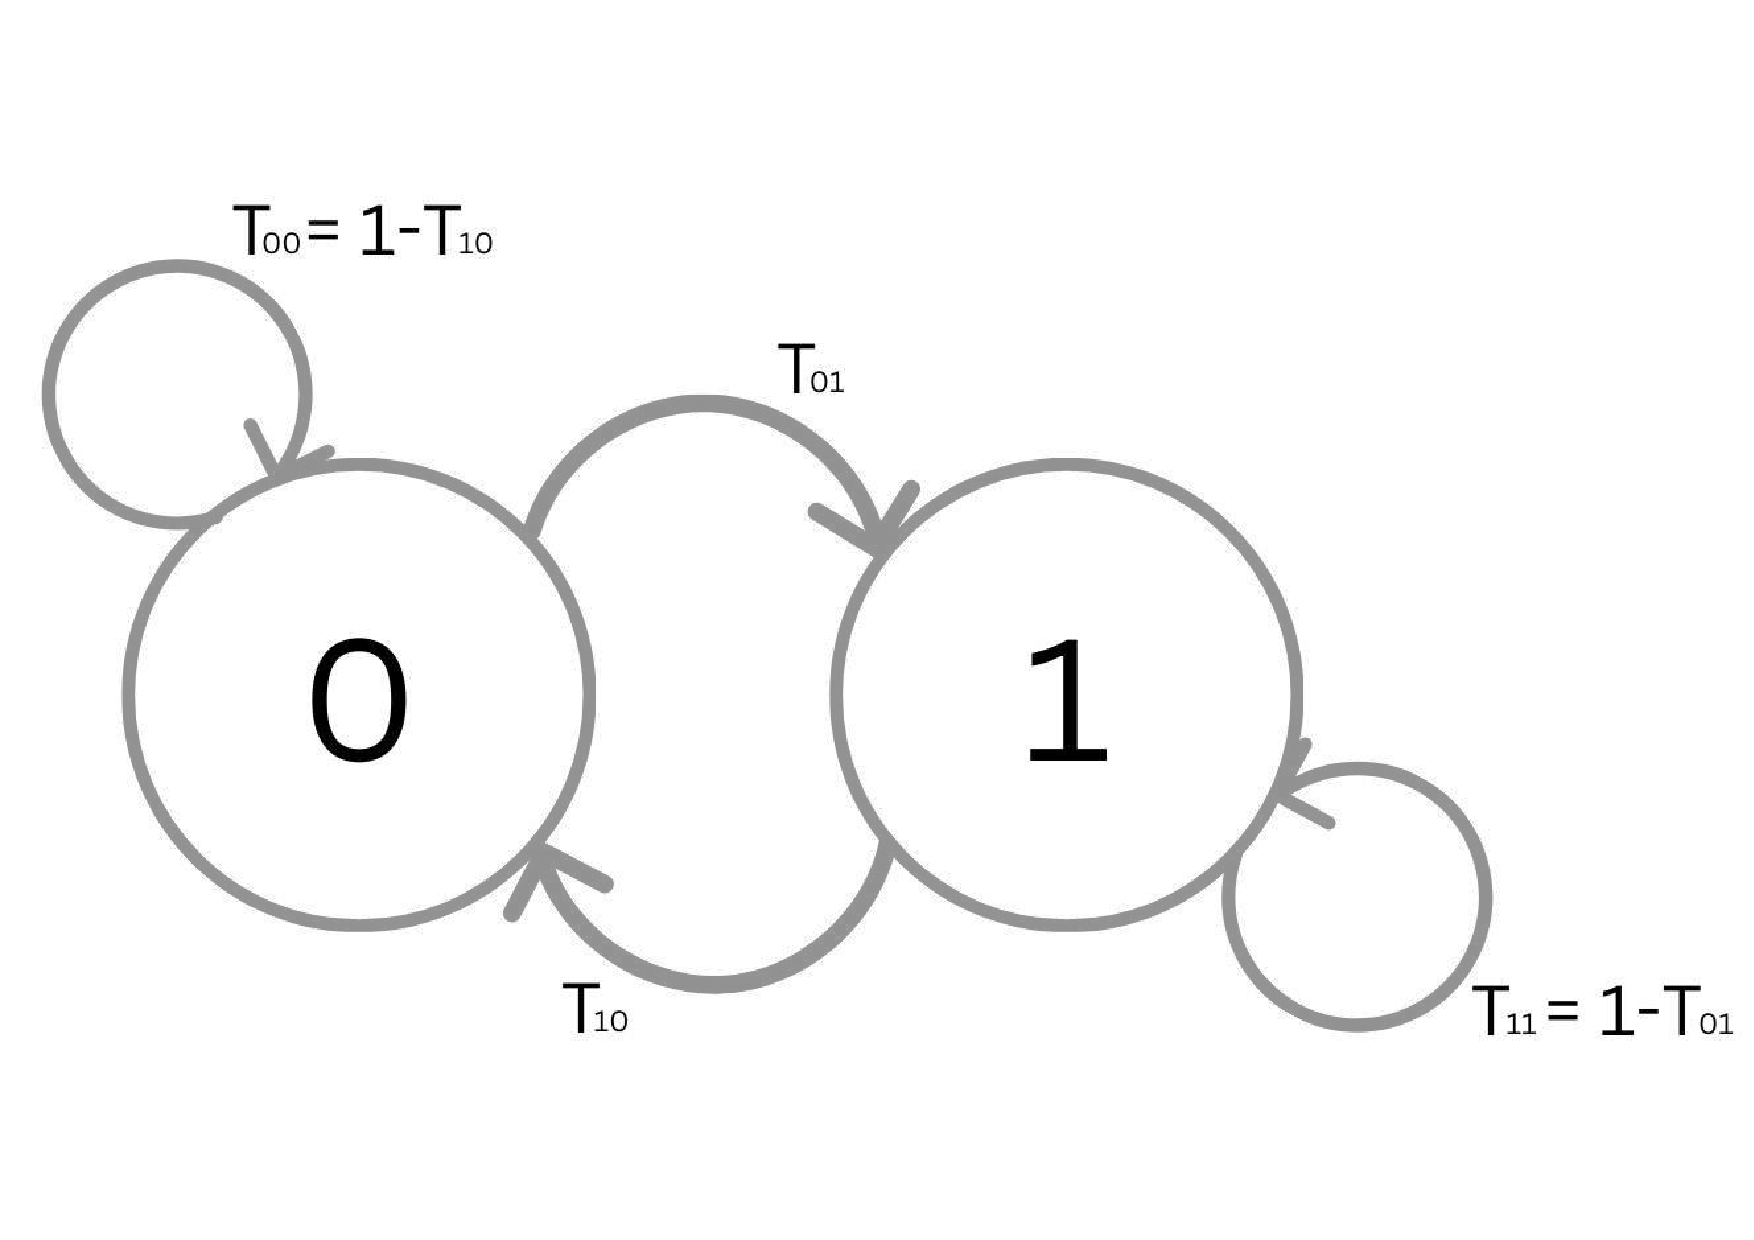
\includegraphics[width=\textwidth]{figures/MKV1.pdf}
        \caption{Diagram of Markov Chain with states of 1-bit}
        \label{fig:MKV1}
    \end{minipage}
    \hfill
    \begin{minipage}{0.45\textwidth}
        \centering
        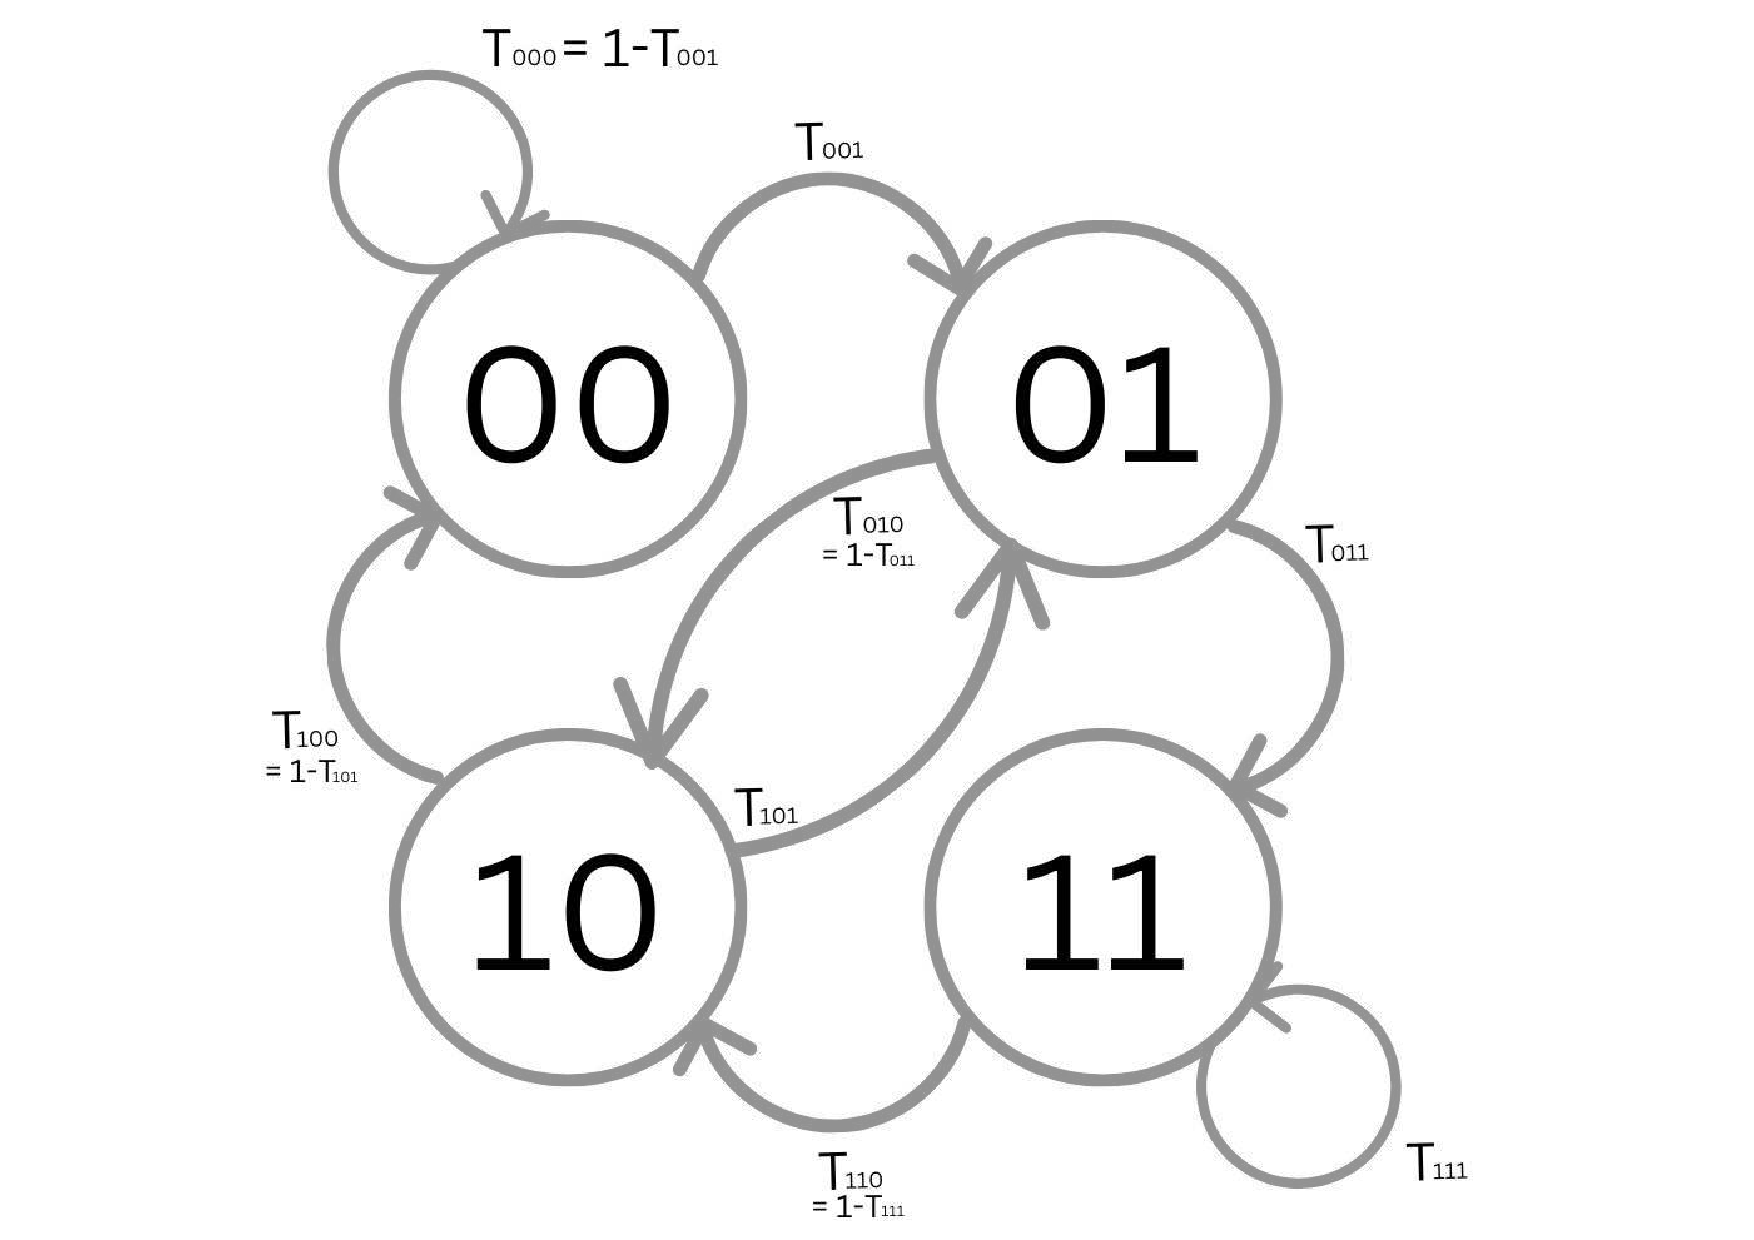
\includegraphics[width=\textwidth]{figures/MKV2.pdf}
        \caption{Diagram of Markov Chain with states of 2-bit}
        \label{fig:MKV2}
    \end{minipage}
\end{figure}

If we increase \( M \) to 2, we can have the 2-bit Markov chain model that has four states, and it is illustrated in Fig. \ref{fig:MKV2}.


Transition probabilities are denoted with \( T_{ijk} \), where the two states of 2 bits are \( ij \) and \( jk \), with \( j \) being an overlapped bit. For example, \( T_{010} \) is the probability of transition from state \( 01 \) to \( 10 \).

The post-processing technique that uses the above-mentioned principle of Markov chains to remove or reduce the correlation in the input can be achieved through \textbf{inverting the operation that generates the bitstring}, where \( M \) now represents the history size.

\begin{figure}[h]
    \centering
    \begin{minipage}{0.45\textwidth}
        \centering
        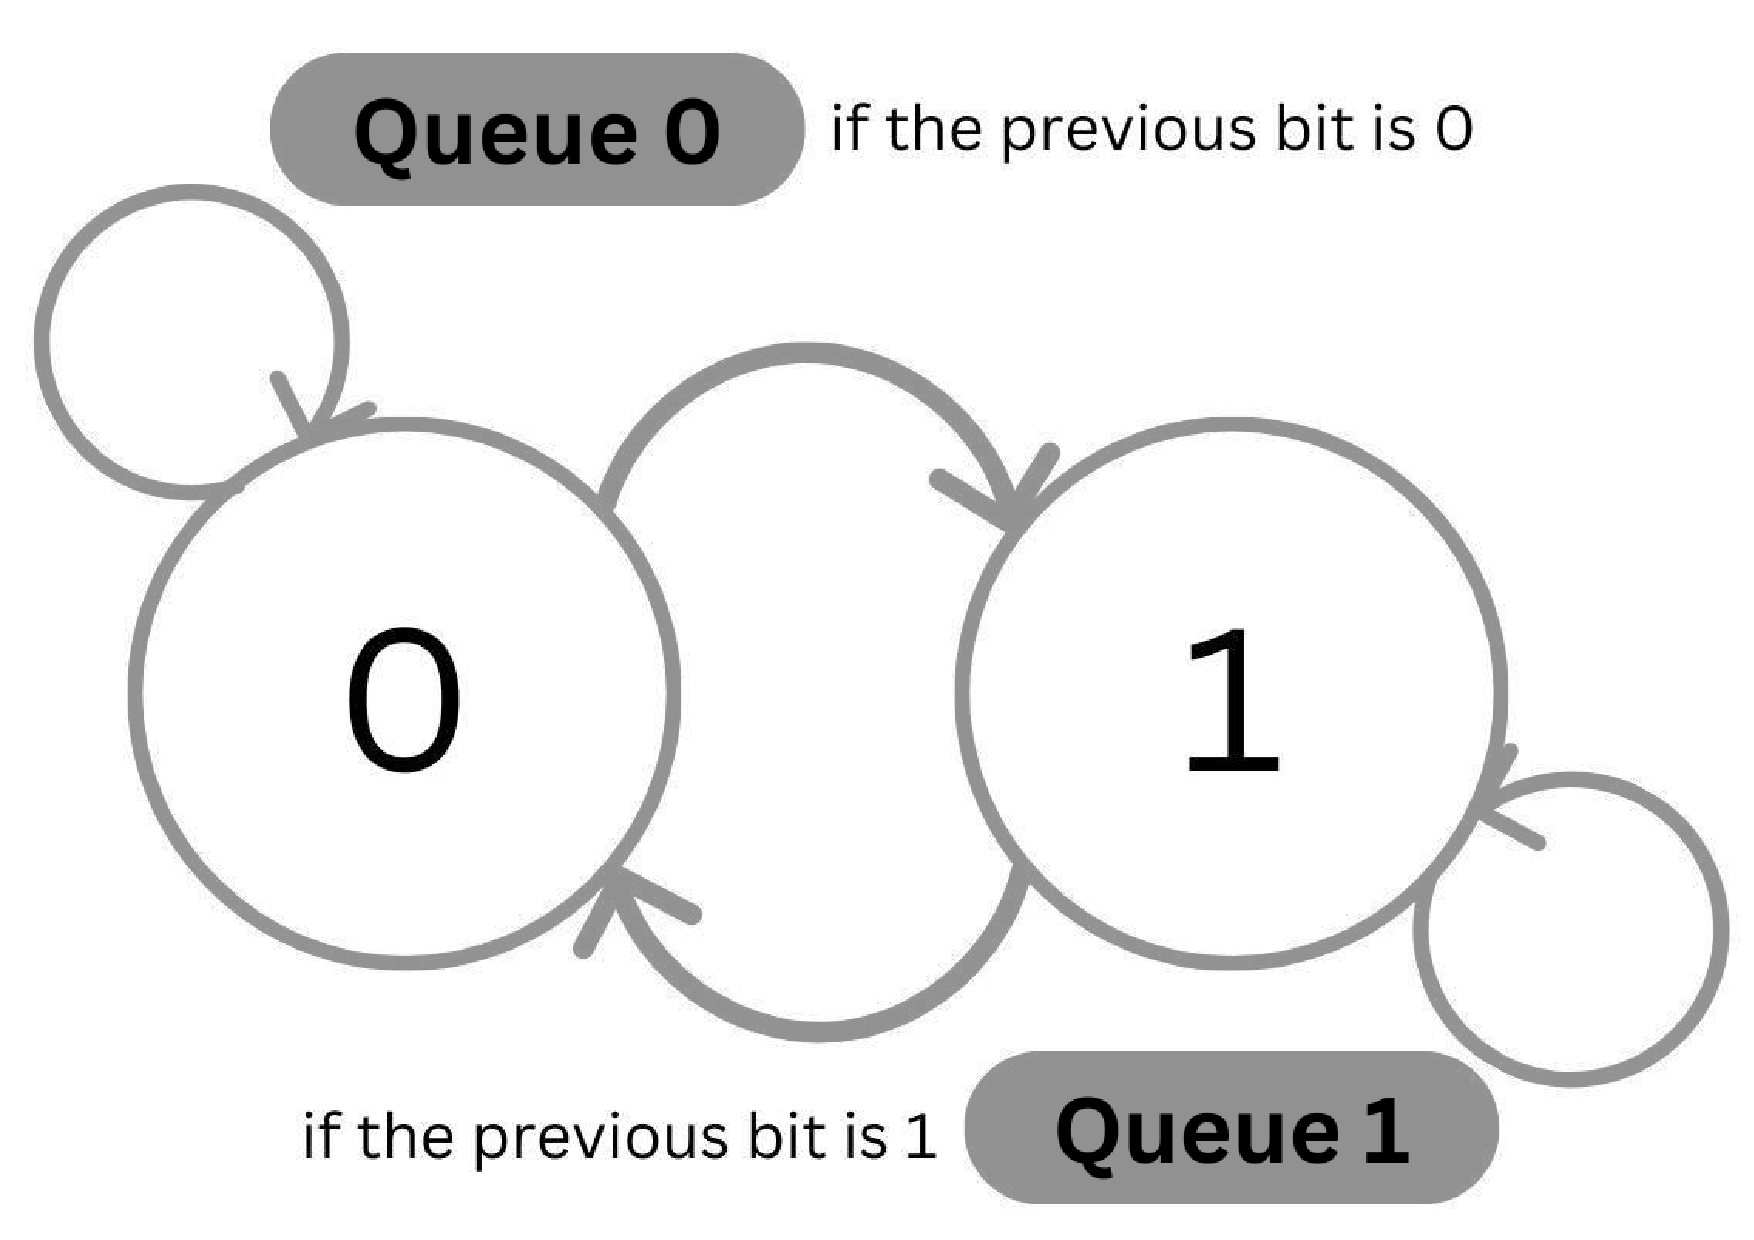
\includegraphics[width=\textwidth]{figures/mkv1 model.pdf}
        \caption{Diagram of Markov Chain de-correlation with 1-bit history}
        \label{fig:MKV22}
    \end{minipage}
    \hfill
    \centering
    \begin{minipage}{0.45\textwidth}
        \centering
        \includegraphics[width=\textwidth]{figures/MKV2_MODEL.pdf}
        \caption{Diagram of Markov Chain with states of 2-bit}
        \label{fig:MKV2mod}
    \end{minipage}
    
\end{figure}

The correlated input bitstream is routed using a Markov chain with \( M \)-bit history to \( 2^M \) queues:

For instance, \( M=1 \):  
The first bit is directly routed to the output.  
Starting from the second bit, if the previous one is 0, the bit is saved in \( \text{Queue}_0 \), and if it is 1, the bit is saved in \( \text{Queue}_1 \).  
At the end, we concatenate the two decorrelated queues (the order is not important).  
We can see the Markov de-correlation model in Fig. \ref{fig:MKV22}.


The entire process of the post-processor is illustrated in Fig. \ref{fig:MKVpp2}.

\begin{figure}
\centering
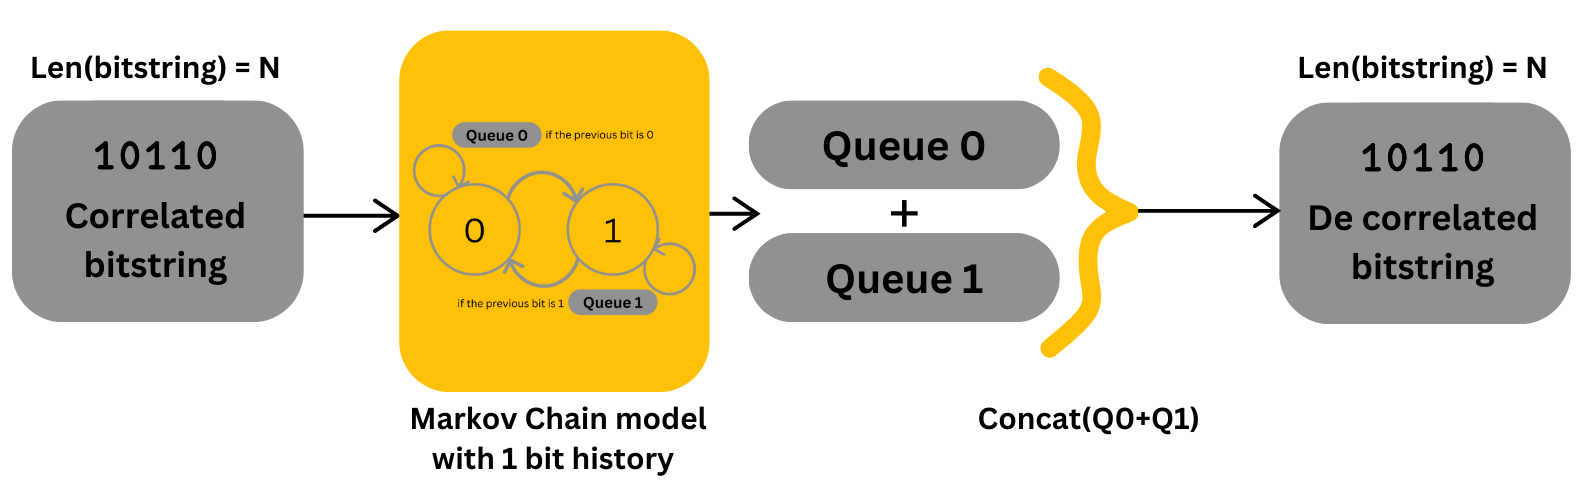
\includegraphics[width=16cm]{figures/De-Cor.png}\vspace{-0.2cm}
\caption{Post-Processing Method process using Markov Chain with 1-bit history and 2 queues}
\label{fig:MKVpp2}
\end{figure}



For instance, \( M=2 \):  
The first two bits are directly routed to the output.  
Starting from the third bit, if the previous two bits are \( 00 \), the bit is saved in \( \text{Queue}_{00} \), and so on.  
At the end, we concatenate the four decorrelated queues (the order is not important).  
We can see the Markov de-correlation model in Fig. \ref{fig:MKV2mod}.



The entire process of the post-processor that uses 2-bits history is illustrated in Fig. \ref{fig:MKV2dd}. 


\begin{figure}
\centering
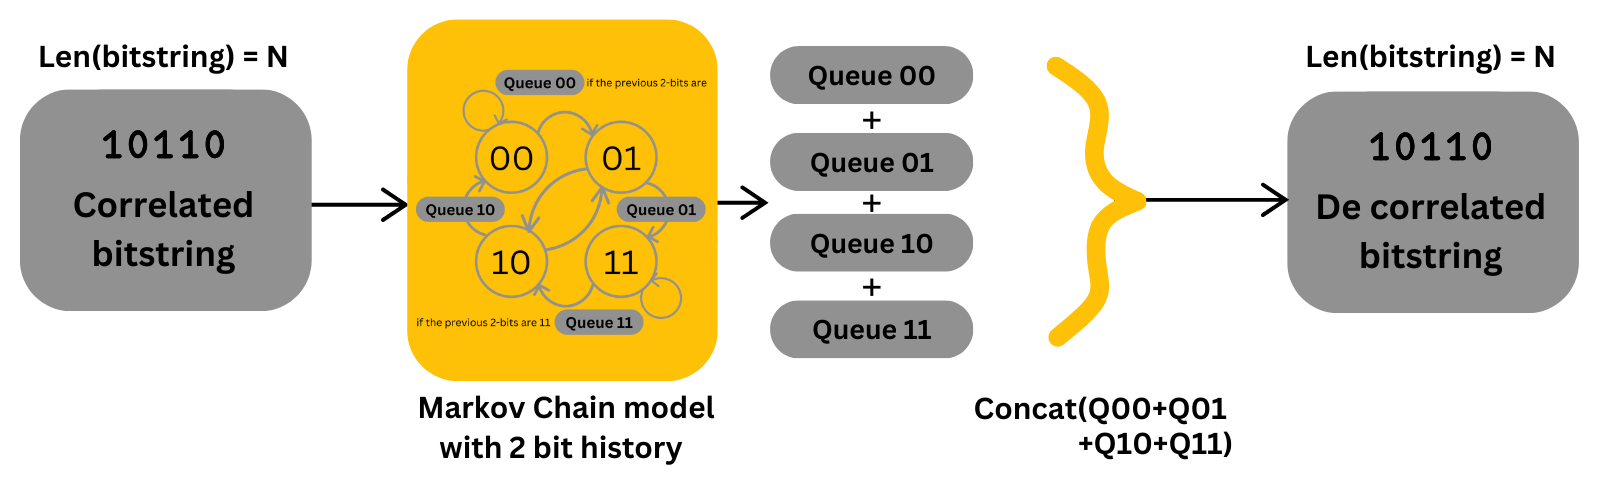
\includegraphics[width=16cm]{figures/De-Cor 2.png}\vspace{-0.2cm}
\caption{Post-Processing Method process using Markov Chain with 2-bits history and 4 queues}
\label{fig:MKV2dd}
\end{figure}

This scheme scores well in reducing the autocorrelation from the input, but since it discarded no bits, and the same length and bits are preserved, the bias of the bitstring and its entropy will not be improved.

A method to combine the properties of de-biasing from the Von Neumann PP and de-correlation from the Markov Chain PP was proposed by Zhang et al. in \cite{dede}, where the results were promising for different Markov models and randomly generated bitstrings, successfully passing most of the randomness tests, The diagram of the proposed flow is illustrated in Fig. \ref{fig:zhang}

\textbf{\textit{Note: The implementation of the Markov Model Bitstring Generation, and Markov Chain De-Correlation and Post Processing functions in python are included in the Appendecies}}


\begin{figure}
\centering
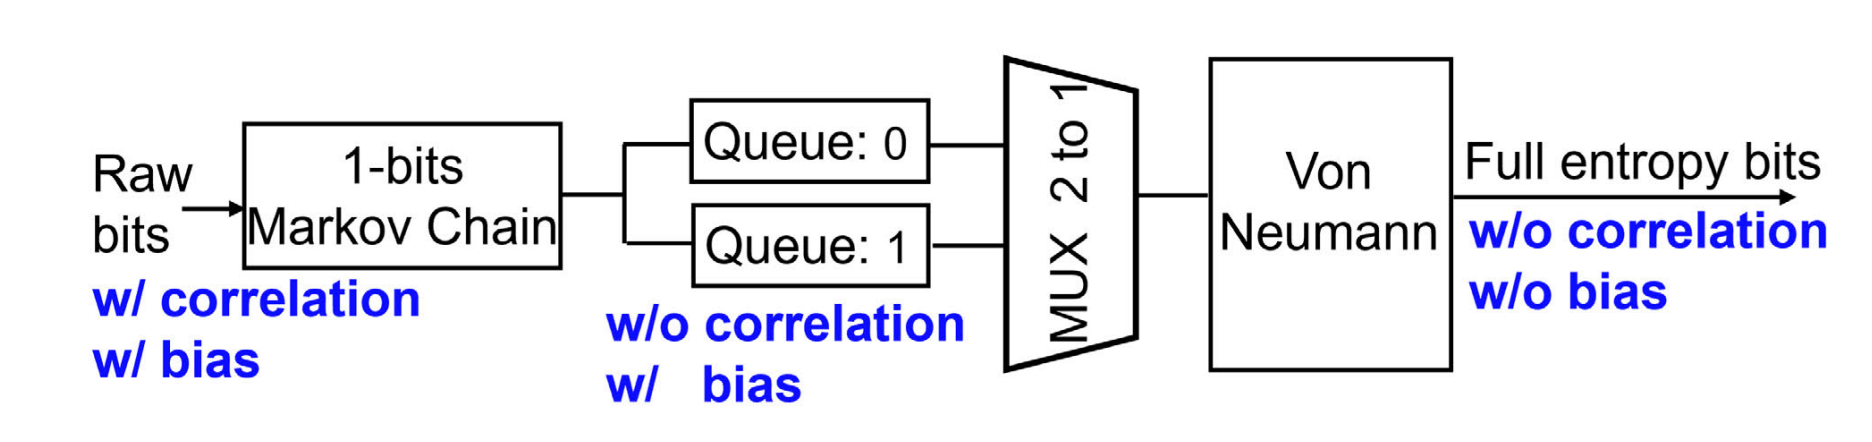
\includegraphics[width=16cm]{figures/ZHANG.png}\vspace{-0.2cm}
\caption{Diagram of de-correlation and de-bias by Markov chain and von
Neumann post-processing proposed by Zhang et Al in \cite{dede}}
\label{fig:zhang}
\end{figure}

\section{The Purpose And Goal of this Work \& Study}
In the previous subsections, we revisited the core principles surrounding True Random Number Generators (TRNGs) and explored various methods to improve the random but defective and imperfect output generated by physical entropy sources. We also listed the shortcomings of these methods.

The primary purpose of this study is to introduce and analyze a new post-processing method, hereby called the CQT Post Processor (CQTPP), along with its variants. This method aims to overcome the Von Neumann method's inability to handle dependent (autocorrelated) bitstreams. Additionally, we benchmark its results against other post-processing techniques using different hyperparameters to evaluate its performance in extracting true randomness from quantum entropy sources.

Special attention will be given to the Boson Sampling as an entropy source introduced in \cite{shi_Twa3na}, whose features in terms of randomness and sampling applications will be explored. Finally, we introduce a Python package, named CQT\_RNG, which integrates all these properties, methods, and metrics that were and will be discussed in this work
 






